% \documentclass{report}
% 
% \usepackage{fancyhdr}
\usepackage{fourier-orns}
\usepackage{hyperref}%% To refrence links / jumps
\usepackage{chngcntr} %% For some extra counters numberings
\usepackage[a4paper, right = 0.5in, left = 0.5in,top = 1in , bottom = 1in]{geometry}
\usepackage{etoolbox} %% Provides like a language for advanced customization
\usepackage{datetime} %% For dates of course
\usepackage{lastpage} %% provides pages numbers
\usepackage[sc]{titlesec} %% modify titles
\usepackage{enumerate}
\usepackage{cancel}
\usepackage{tikzsymbols}
\usepackage[dvipsnames]{xcolor}
\usepackage{import}
\usepackage{pdfpages} %% include other pdfs
\usepackage{transparent} %% Transparency
\usepackage{xcolor}  %% Colors
\usepackage[many]{tcolorbox}
\usepackage[framemethod=TikZ]{mdframed}
\usepackage{amsmath,amsfonts,amsthm,amssymb,mathtools}
\usepackage{tikz}
\usepackage{bookmark}
\usepackage{graphicx}
\usepackage{mathpazo}

\usepackage{fontawesome5}

\linespread{1.5}


\titleformat{\chapter}[display]   
{\fontfamily{ppl}\selectfont\huge\color{YellowOrange!80!orange}} % Font style and size 
{\raggedleft\color{purple}\fontsize{70}{0pt}\selectfont\thechapter}   
{-1.5cm}    			                          % Space between the chapter number and title
{
	\begin{tikzpicture}[overlay]
		\node[anchor = west,yshift = 0.2cm,xshift = -1cm] {\fontsize{90}{20} $\int_{}^{} $};
		\node[yshift = 4cm, xshift = 17cm]   {\includegraphics[width = 4cm]{preview0}};
	\end{tikzpicture}
\hspace{1cm}\Huge\raggedright\MakeUppercase}

\titleformat{\section}[block]
{
\fontfamily{ppl}\selectfont\huge\color{YellowOrange!80!orange}
}
{
\color{purple}\fontsize{20}{0pt}\selectfont\thesection 
}
{0cm}
{
	\begin{tikzpicture}[overlay]
		\node[anchor = west,yshift = 0.2cm,xshift = -0.4cm, circle = 1pt] {};
	\end{tikzpicture}
}

\titlespacing*{\section}{0pt}{0.7cm}{1.5cm}


\newcommand{\divider}
{
	\begin{center}
	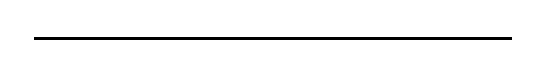
\begin{tikzpicture}
		\draw[thick, black] (0.25*\textwidth, 0) -- (0.75*\textwidth, 0);
		\node[rotate = 360 - 90, xshift = -0.6pt, yshift = 1pt] at (0.25*\textwidth,0){\decotwo};
		\node[rotate = 90, xshift = -0.6pt, yshift = 1pt] at (0.75*\textwidth,0){\decotwo};
	\end{tikzpicture}
	\end{center}
}

\pagestyle{fancy}

\newcommand{\lecday}[1][]
{
    \def\datee{#1}
    \fancyhead[L]{\datee}
}



\newcommand{\signature}
{
	\begin{tikzpicture}[remember picture,overlay]
		\node[fill = YellowOrange!20!white] at ([yshift = 1cm, xshift = -3cm]current page.south east) {\fontsize{10pt}{0pt}{\itshape Kara.$\mathcal{A}$}};
	\end{tikzpicture}
}

\AddToHook{shipout/background}{
  \begin{tikzpicture}[remember picture, overlay]
	  \node[] at ([yshift = 1.5cm,xshift = \textwidth /2 + 0.9cm]current page.south west) {\includegraphics[width = 0.5cm]{preview3}};
	  \node[] at ([yshift = 1.5cm,xshift = - \textwidth /2 - 0.9cm]current page.south east) {\includegraphics[width = 0.5cm]{preview4}};
  \end{tikzpicture}
}



\newtcolorbox[auto counter, number within = section]{remark}[1][]
{
       		title = Remark #1,
		enhanced,
		boxrule = 0pt,
		colback = white,
		breakable,
		arc = 4pt,
		colbacktitle = cyan,
		colback = cyan!5!white,
		segmentation style =
		{
			solid,cyan,thick,
		},
		attach boxed title to top left =
		{
			xshift = 0cm,
		},
		boxed title style =
		{
			boxrule = 0pt,
			sharp corners,
			drop fuzzy shadow = {cyan},
		},
		drop fuzzy shadow = {cyan!80!black},
}

\newtcolorbox[auto counter, number within = section]{theorem}[1][]
{                                      
		title = Theorem \thetcbcounter : #1,
		enhanced, 
		boxrule = 0pt,
		colback = white,
		breakable,
		arc = 4pt,
		colbacktitle = purple,
		colback = purple!5!white,
		segmentation style = 
		{
			solid, purple,thick,
		},
		attach boxed title to top left = 
		{
			xshift = 0cm, 
		},
		boxed title style = 
		{
			boxrule = 0pt,
			sharp corners,
			drop fuzzy shadow = {purple},
		},
		drop fuzzy shadow = {purple!80!black},
}

\newtcolorbox[auto counter, number within = section]{definition}[1][]
{                                      
		title = Definition \thetcbcounter : #1,
		enhanced, 
		boxrule = 0pt,
		colback = white,
		arc = 4pt,
		breakable,
		colbacktitle = YellowOrange!80!black,
		segmentation style = 
		{
			solid, YellowOrange,thick,
		},
		attach boxed title to top left = 
		{
			xshift = 0cm, 
		},
		colback = YellowOrange!5!white,
		boxed title style = 
		{
			boxrule = 0pt,
			sharp corners,
			drop fuzzy shadow = {YellowOrange!80!orange},
		},
		drop fuzzy shadow = {YellowOrange!80!black},
}

\newtcolorbox[auto counter, number within = section]{corollary}[1][]
{                                      
		title = corollary \thetcbcounter : #1,
		enhanced, 
		boxrule = 0pt,
		colback = white,
		arc = 4pt,
		breakable,
		colbacktitle = YellowOrange!80!black,
		segmentation style = 
		{
			solid, YellowOrange,thick,
		},
		attach boxed title to top left = 
		{
			xshift = 0cm, 
		},
		colback = YellowOrange!5!white,
		boxed title style = 
		{
			boxrule = 0pt,
			sharp corners,
			drop fuzzy shadow = {YellowOrange!80!orange},
		},
		drop fuzzy shadow = {YellowOrange!80!black},
}


\newtcolorbox{example}[1][]
{                                      
		title = Example,
		enhanced, 
		boxrule = 0pt,
		colback = white,
		arc = 4pt,
		segmentation style = 
		{
			solid, SpringGreen,thick,
		},
		breakable,
		colback = SpringGreen!5!white,
		colbacktitle = SpringGreen!80!black,
		attach boxed title to top left = 
		{
			xshift = 0cm, 
		},
		boxed title style = 
		{
			boxrule = 0pt,
			sharp corners,
			drop fuzzy shadow = {SpringGreen!80!orange},
		},
		drop fuzzy shadow = {SpringGreen!80!black},
}


\newcommand{\integral}[4]{\int\limits_{#1}^{#2} #4 d#3}
\newcommand{\limit}[3]{\lim\limits_{#1 \rightarrow #2} #3}
\newcommand{\strone}[2]{\left[ \begin{gathered}#1\\ #2\end{gathered} \right] }
\newcommand{\strtwo}[2]{\left\{ \begin{gathered}#1\\ #2\end{gathered} \right\} }
\newcommand{\strthree}[2]{\left\lfloor \begin{gathered}#1\\ #2\end{gathered} \right\rfloor }


\newcommand{\startbf}[1]{\text{\bfseries{#1}}}
\newcommand{\sett}[1]{\left\{ #1 \right\}}
\newcommand{\thesis}[1]{\left( #1 \right)}
\newcommand{\brkt}[1]{\left[ #1 \right]}
\newcommand{\floor}[1]{\left\lfloor #1 \right\rfloor}


\DeclareMathOperator{\img}{im} % Image
\DeclareMathOperator{\Img}{Im} % Image
\DeclareMathOperator{\coker}{coker} % Cokernel
\DeclareMathOperator{\Coker}{Coker} % Cokernel
\DeclareMathOperator{\Ker}{Ker} % Kernel
\DeclareMathOperator{\rank}{rank}
\DeclareMathOperator{\Spec}{Spec} % spectrum
\DeclareMathOperator{\Tr}{Tr} % trace
\DeclareMathOperator{\pr}{pr} % projection
\DeclareMathOperator{\ext}{ext} % extension
\DeclareMathOperator{\pred}{pred} % predecessor
\DeclareMathOperator{\dom}{dom} % domain
\DeclareMathOperator{\ran}{ran} % range
\DeclareMathOperator{\Hom}{Hom} % homomorphism
\DeclareMathOperator{\Mor}{Mor} % morphisms
\DeclareMathOperator{\End}{End} % endomorphism


\newcommand{\lm}{\ensuremath{\lambda}}
\newcommand{\eps}{\ensuremath{\epsilon}}
\newcommand{\veps}{\ensuremath{\varepsilon}}
\newcommand{\al}{\ensuremath{\alpha}}
\newcommand{\bb}{\ensuremath{\beta}}
\newcommand{\cc}{\ensuremath{\gamma}}
\newcommand{\dd}{\ensuremath{\delta}}
\newcommand{\DD}{\ensuremath{\Delta}}
\newcommand{\ff}{\ensuremath{\phi}}
\newcommand{\FF}{\ensuremath{\varphi}}

\newcommand{\RR}{\mathbb{R}}
\newcommand{\RO}{\mathcal{R}}
\newcommand{\EE}{\mathbb{E}}
\newcommand{\CC}{\mathbb{C}}
\newcommand{\RW}{\mathbb{R}^2}
\newcommand{\RT}{\mathbb{R}^3}
\newcommand{\RN}{\mathbb{R}^n}
\newcommand{\DS}{\mathcal{D}}

\newcommand{\KK}{\mathbb{K}}
\newcommand{\KW}{\mathbb{K}^2}
\newcommand{\KT}{\mathbb{K}^3}
\newcommand{\KN}{\mathbb{K}^n}

\newcommand{\NN}{\mathbb{N}}

\newcommand{\PS}{\mathcal{P}}
\newcommand{\AS}{\mathcal{E}}
\newcommand{\FS}{\mathcal{F}}
\newcommand{\LS}{\mathcal{L}}
\newcommand{\MS}{\mathcal{M}}

















% 
\lecday[2025-04-08]

% \begin{document}
	\divider	
	\lefthand ~\it Recall \normalfont
                Let $E $ be a N.V.S 
		$\sum_{n=0}^{\infty}  x_{n} $ is unconditionally convergent 
		if and only if 
		$\forall  $  $ \sigma    : \NN \longrightarrow \NN $ a bijective, 
		the series $\sum_{n=0}^{\infty}  x_{\sigma (n)   } $ is convergent to the same
		sum.
	\divider	
	\begin{example}
	In $\RR  $, the series,
	\[
	\frac{1}{1} - \frac{1}{2} + 
	\frac{1}{3} - 
	\frac{1}{4} + \hdots 
	\]
	which is convergent to $\ln{(2) } $, is conditionally convergent, consider the permutation of 
	$\NN$, that is given by, 
	\[
		(1, 2, 3, 5, 4, 7, 9, 11, 6, \hdots ) 
	\]
	therefore it transforms to 
	\[
	\frac{1}{1} - \frac{1}{2} + \frac{1}{3} + \frac{1}{5} - \frac{1}{4} + \frac{1}{7} + 
	\frac{1}{9} + \frac{1}{11} - \frac{1}{6} + \hdots 
	\]
	transform it to a divergent series also the permutation, 
	\[
		(1, 2, 4, 3, 6, 8, \hdots )  = (n, 2n, 2n+2)  
	\]
	transforms the series to, 
	\begin{align*}
		\frac{1}{1} - \frac{1}{2} - \frac{1}{4}+  \frac{1}{3} - \frac{1}{6} - \frac{1}{8} + \hdots  &=
	\sum_{n=0}^{\infty}  \left( 
	\frac{1}{2n+1} - \frac{1}{2(2n+1) } - \frac{1}{2(2n+2) }\right) \\ 
&= \sum_{n=0}^{\infty}  \left( \frac{1}{2(2n+1) } - \frac{1}{2(2n+2) } \right) \\
&= \frac{1}{2} \sum_{n=0}^{\infty}  \frac{1}{2n+1} - \frac{1}{2n+2} \\
&= \frac{1}{2}
\left[ 
	\frac{1}{1} - \frac{1}{2} + \frac{1}{3} - \frac{1}{4} + \frac{1}{5} + \hdots 
\right] \\
&= \frac{1}{2} \ln{(2)} \neq  \ln{(2)}
	\end{align*}
	\end{example}
	\begin{theorem}[The Riemann rearrangement]
		If a real series is conditionally convergent 
		then its terms can be rearranged so that the new series converges
		to an arbitrary real number, or diverges
	\end{theorem}
	\begin{theorem}[]
	Let $E $ be a Banach space, then any normally convergent series of $E $ is unconditionally
	convergent 
	\end{theorem}
	\begin{proof}
	Let $\sum_{n=0}^{\infty}  x_{n} $  be a normally convergent series of $E $ (i.e. 
	the real series $\sum_{n=0}^{\infty}  \| x_{n} \|  $ is convergent), then 
	for the permutation $\sigma  : \NN \longrightarrow \NN $ we have for all $n\in  \NN$, 
	we will consider the series,
	\begin{align*}
		\sum_{n=0}^{N}  \| x_{\sigma (n)   }   \|  = 
		\sum_{k \in  
		\left\{ \sigma (0) , \hdots , \sigma (N)      \right\}}^{}  
		\| x_{k} \|  &\leq 
		\sum_{k=1}^{\max (\sigma (i)   ) , 1 \leq i \leq N} 
		\| x_{k} \|  \\
	     & \leq 
	     \sum_{k=1}^{\infty } \| x_{k} \|  \\
	\end{align*}
	This implies that the nonegative real series $\sum_{n=0}^{\infty}  \| x_{\sigma (n)   } \|  $ 
	is convergent, that is the series $\sum_{n=0}^{\infty}  x_{\sigma (n)   }$ of $E $ is
	normally convergent, since $E $ is Banach so we conclude that the series 
	$\sum_{n=0}^{\infty}  x_{\sigma (n)}$ is convergent, as required.\\
	Now let us show that $\sum_{n=0}^{\infty}  x_{\sigma (n)   } $  
	has the same sum as $\sum_{n=0}^{\infty}  x_{n} $  
	let us define for all $n \in \NN $. 
	\[
	a_{n} = 
	\begin{cases}
		 \min \left( A = \left\{ 1, 2, \hdots ,n  \right\} \DD  
		\left\{ \sigma (1) , \hdots , \sigma (n)      \right\}\right)  
		\\
		n
	\end{cases} 
	\begin{gathered}  
		\text{ if } A \neq \emptyset   \\  
		\text{ if }   A = \emptyset 
	\end{gathered}
	\]
	and let us admit for the moment that 
	\[
	\lim_{n \to \infty} a_{n} = \infty 
	\]
	then we have for all $n \in \NN $, 
	\begin{align*}
		\| \sum_{n=1}^{N} x_{\sigma (n)   }- \sum_{n=1}^{N} x_{n} \| &=
		\| \sum_{i \in \left\{ 
		\sigma (1) , \hdots , \sigma (n)     \right\}}^{} x_{i} - 
		\sum_{i \in \left\{ 1, \hdots , N \right\}}^{} x_{i}\|  \\
									     &= 
					\| \sum_{i \in 
					\left\{ \sigma (1) , \hdots , 
				\sigma (N)   \right\} \backslash 
		\left\{ 1,2, \hdots , N \right\}}^{} x_{i} - 
		\sum_{i \in \left\{ 1, \hdots , N \right\} \backslash 
		\left\{ \sigma (1) , \hdots , \sigma (N)      \right\}}^{} \| 
		\\
									     & \leq 
				\sum_{i \in \left\{ \sigma (1) , \hdots , \sigma (N) \right\} \backslash 
			\left\{ 1, \hdots , N \right\}}^{}
			\| x_{i} \|  + 
			\sum_{i \in  \left\{1, \hdots , N  \right\} \backslash 
		\left\{ \sigma (1) , \hdots , \sigma (N)      \right\}}^{}  
		\| x_{i} \| \\
									     &=
		\sum_{i \in  \left\{ 1, \hdots , N \right\} 
		\DD \left\{ \sigma (1) , \hdots , \sigma (N)      \right\}}^{}  
		\| x_{i} \|  \\
									     & \leq 
		\sum_{i \geq a_{N}}^{}  \| x_{i} \| 
	\end{align*}
	Then by letting $N \rightarrow \infty  $, we get since $\sum_{i=1}^{\infty } \| x_{i} \|  $ 
	converge and 
	$a_{N} \rightarrow \infty  $  as $N \rightarrow \infty  $,  we get, 
	\[
	\sum_{n=0}^{\infty}  x_{\sigma (n)   } = 
	\sum_{n=0}^{\infty}  x_{n}
	\]
	as required. \\
	Now, it remains to prove that $\lim_{n \to \infty} a_{n} =\infty  $, this is equivalent
	to show that for all $k \in \NN $, there exist $N_{k} $ such that $\forall n \in \NN : 
	n \geq N_{k} \implies a_{n} \geq k$, now let $k \in \NN $, and take $N_{k} :=
	\max \left\{ 1, \hdots , k, 
	\sigma ^{-1}(1) , \hdots , \sigma ^{-1}(k)  \right\}$, then for any $n \in \NN $, we have in 
	one hand: 
	\[
	N \geq N_{k} \implies 
	N \geq k \quad \text{ ( since $N_{k} \geq k $  )}   \implies 
	\left\{ \sigma (1) , \hdots , \sigma (N)   \right\} \backslash 
	\left\{ 1, \hdots , N \right\} \subset 
	\left\{ k+1, k+2, \hdots   \right\} 
	\]
	On the other hand, 
	\[
	N \geq N_{k} \implies 
	\sigma \sigma ^{-1}(1), \sigma ^{-1}(2), \hdots , \sigma ^{-1}  (k)  \leq  N_{k} \leq N
	\]
	which implies, 
	\begin{align*}
	& \implies 	\sigma ^{-1}(1) , \sigma ^{-1}(2) , \hdots , \sigma ^{-1}(k)   
		\in \left\{ 1, \hdots , N \right\} \\
	& \implies 
	1, \hdots , k \in  \left\{ \sigma (1) , \hdots , \sigma (N)      \right\} \\
	& \implies 
	\left\{ 1, \hdots , N \right\} \backslash 
	\left\{ \sigma (1) , \hdots , \sigma (N)      \right\} \subset 
	\left\{ k+1, k+2, \hdots  \right\} 
	\end{align*}
	so from the two hands, we get $\forall n \in \NN $, 
	\begin{align*}
		N \geq N_{k} & \implies 
		\left\{ 1, \hdots, N \right\} \DD 
		\left\{ \sigma (1) , \hdots , \sigma (N)      \right\} \subset 
		\left\{ k+1, k+2, \hdots  \right\} \\
			     & \implies 
			     a_{N} \geq k \quad 
			     \text{ (also true for $ a_{N} = N$, since $N \geq N_{k} \geq k $)} 
	\end{align*}
	as required. Thus $a_{n} \rightarrow  \infty  $ as $n \rightarrow \infty  $. which completes
	the proof.
	\end{proof} 
	\section{The summability of general series}
	We call a general series any infinite sum of element of a N.V.S, that is a 
	$\sum_{i \in I}^{} x_{i} $, where $I $ is infinite.
	\begin{definition}[Generalize the unconditional convergence]
		Let $E $ be a N.V.S. A general series $\sum_{i \in I}^{} x_{i} $ of $E $ 
		is said to be summable with sum $S \in E $, if it satisfies the following property, 


		$\forall \veps  > 0, \exists I_{\veps } \subset I $ finite, s.t. 
		$\forall  J $ a finite subset of $I $, we have 
		\[
		I_{\veps } \subset J \implies 
		\| \sum_{i \in J}^{} x_{i} - S \|  < \veps 
		\]
	\end{definition}
	\divider	
	Let $E $ be a N.V.S. If a general series $\sum_{i \in I}^{} x_{i} $ is 
	summable then it has a unique sum,
	\begin{proof}
	Let $\sum_{i \in I}^{} x_{i} $ be a general summable series with sums $S $  and $S' $ 
	$(S, S' \in E)  $, and let us prove that $S = S' $. Let $\veps  > 0 $ arbitrary, By definition
	$\exists I_{\veps } \subset I $, with $I_{\veps } $ finite, such that, 

	$\forall J $ a finite subset of $I$, we have 
	\[
	I_{\veps } \subset J \implies 
	\| \sum_{i \in J}^{} x_{i} - S \|  < \frac{\veps }{2} 
	\]
	Similarly, $\exists I_{\veps } \subset I $, with $I_{\veps } $ finite, such that 

	$\forall J $ a finite subset of $I $, we have, 
	\[
	I_{\veps } \subset 
	J \implies 
	\| \sum_{i \in J}^{} x_{i} - S'  \|  < \frac{\veps }{2}
	\]
	So, by taking $J = I_{\veps }\cup I_{\veps }' $ which if a finite subset of $I $ and contains 
	both $I_{\veps } $ and $I_{\veps }' $, we have, 
	$\| \sum_{i \in  J}^{} x_{i} - S \|   <  \frac{\veps }{2}$  and 
	$\| \sum_{i \in J}^{} x_{i} - S' \|  <  \frac{\veps }{2} $. Hence, 
	\begin{align*}
		\| S - S' \|  &= 
		\| S - \sum_{i \in J}^{} x_{i} + \sum_{i \in J}^{} x_{i} - S' \|  \\
			      & \leq 
			      \| S - \sum_{i \in J}^{} x_{i} \|  + 
			      \| \sum_{i \in J}^{} x_{i} - S' \|  < 
			      \frac{\veps }{2} + \frac{\veps }{2} \quad 
			      \quad (= \veps ) 
	\end{align*} 
	Thus $\| S - S' \|  <  \veps  $ for all $ \veps  > 0 $, implying that  
	$S = S' $, as required.
	\end{proof}
	\divider
	\begin{center}
		\it The Cauchy Criterion \normalfont
	\end{center}
	Let $E $ be a N.V.S. We say that a general series $\sum_{i \in I}^{} x_{i} $. Satisfies 
	the Cauchy Criterion if,  


	$\forall \veps  > 0,\exists I_{\veps } \subset I$, with 
	$I_{\veps } $ finite, s.t. $\forall J $ a finite subset of $I $, disjoint with $I_{\veps } $,
	we have 
	\[
	\| \sum_{i \in J}^{} x_{i} \|  <  \veps 
	\]
	\divider 
	$\sum_{i \in \NN}^{} x_{i} $  is Cauchy if and only if 
	\[
	\forall  \veps  >  0, \exists  N_{\veps } \in \NN \text{ s.t. }  
	\forall  p,q \in  \NN: p > q > N_{\veps } \implies 
	\| \sum_{i=q+1}^{p} x_{i}  \|  <  \veps 
	\]
	which implies that 
	\[
	\forall  \veps  > 0, 
	\exists  I_{\veps } = 
	\left\{ 1, \hdots , N_{\veps } \right\} \subset \NN \text{ finite s.t. } 
	\forall  J = \left\{ q+1, \hdots, p \right\} 
	\subset \NN \text{ finite } 
	\]
	and 
	\[
	J \cap I_{\veps } = \emptyset  \implies 
	\| \sum_{i \in J}^{} x_{i} \|  <  \veps 
	\]
	\begin{theorem}[]
	Let $E $ be a Banach Space. 
	Then every general series $\sum_{i \in I}^{} x_{i} $  
	of $E $ which satisfies the cauchy criterion is summable. 
	\end{theorem}
	\begin{proof}
	Let $\sum_{i \in I}^{} x_{i} $ be a general series of $E $. Which satisfies the Cauchy
	criterion then for all $n \in \NN $, there exist $I_{n} \subset I $  with $I_{n} $ finite, 
	such that $\forall  J $ a finite subset of $I $, with $J \cap I_{n} = \emptyset  $, we have 
	$\| \sum_{i \in J}^{} x_{i}  \| <  \frac{1}{n}  $ , let us define for all $n \in \NN $, 
	\[
	S_{n} := 
	\sum_{i \in  I_1 \cup  I_2 \cup  \hdots \cup I_{n} }^{}  x_{i} \quad \quad 
	\text{( a finite sum )} 
	\]
	$(S_{n}) _{n \in \NN} $  is a sequence of $E $\\ 
	we have for any $p,q \in \NN $, with $p > q $, 
	\[
		\| S_{p} - S_{q}  \|  = 
		\| \sum_{i \in
			\underbrace{
			I_{1} \cup \hdots \cup I_{p} \backslash 
		I_{1} \cup \hdots \cup I_{q}
			}_{\text{ disjoint ($I_{p},I_{q}$) } } 
	}^{} x_{i} \|   < \frac{1}{q} \rightarrow 0 \text{ as }  q \rightarrow \infty 
	\]
	Thus $(S_{n}) _{n \in \NN} $ is Cauchy. Since $E $ is Banach then $(S_{n}) _{n \in \NN} $  
	is convergent. Let $S = \lim_{n \to \infty} S_{n} \in E$ , and let us show that 
	the general series $\sum_{i \in I}^{} x_{i} $  is sommable with sum $S$ 
	\end{proof}
% \end{document}
